\documentclass[1p]{elsarticle_modified}
%\bibliographystyle{elsarticle-num}

%\usepackage[colorlinks]{hyperref}
%\usepackage{abbrmath_seonhwa} %\Abb, \Ascr, \Acal ,\Abf, \Afrak
\usepackage{amsfonts}
\usepackage{amssymb}
\usepackage{amsmath}
\usepackage{amsthm}
\usepackage{scalefnt}
\usepackage{amsbsy}
\usepackage{kotex}
\usepackage{caption}
\usepackage{subfig}
\usepackage{color}
\usepackage{graphicx}
\usepackage{xcolor} %% white, black, red, green, blue, cyan, magenta, yellow
\usepackage{float}
\usepackage{setspace}
\usepackage{hyperref}

\usepackage{tikz}
\usetikzlibrary{arrows}

\usepackage{multirow}
\usepackage{array} % fixed length table
\usepackage{hhline}

%%%%%%%%%%%%%%%%%%%%%
\makeatletter
\renewcommand*\env@matrix[1][\arraystretch]{%
	\edef\arraystretch{#1}%
	\hskip -\arraycolsep
	\let\@ifnextchar\new@ifnextchar
	\array{*\c@MaxMatrixCols c}}
\makeatother %https://tex.stackexchange.com/questions/14071/how-can-i-increase-the-line-spacing-in-a-matrix
%%%%%%%%%%%%%%%

\usepackage[normalem]{ulem}

\newcommand{\msout}[1]{\ifmmode\text{\sout{\ensuremath{#1}}}\else\sout{#1}\fi}
%SOURCE: \msout is \stkout macro in https://tex.stackexchange.com/questions/20609/strikeout-in-math-mode

\newcommand{\cancel}[1]{
	\ifmmode
	{\color{red}\msout{#1}}
	\else
	{\color{red}\sout{#1}}
	\fi
}

\newcommand{\add}[1]{
	{\color{blue}\uwave{#1}}
}

\newcommand{\replace}[2]{
	\ifmmode
	{\color{red}\msout{#1}}{\color{blue}\uwave{#2}}
	\else
	{\color{red}\sout{#1}}{\color{blue}\uwave{#2}}
	\fi
}

\newcommand{\Sol}{\mathcal{S}} %segment
\newcommand{\D}{D} %diagram
\newcommand{\A}{\mathcal{A}} %arc


%%%%%%%%%%%%%%%%%%%%%%%%%%%%%5 test

\def\sl{\operatorname{\textup{SL}}(2,\Cbb)}
\def\psl{\operatorname{\textup{PSL}}(2,\Cbb)}
\def\quan{\mkern 1mu \triangleright \mkern 1mu}

\theoremstyle{definition}
\newtheorem{thm}{Theorem}[section]
\newtheorem{prop}[thm]{Proposition}
\newtheorem{lem}[thm]{Lemma}
\newtheorem{ques}[thm]{Question}
\newtheorem{cor}[thm]{Corollary}
\newtheorem{defn}[thm]{Definition}
\newtheorem{exam}[thm]{Example}
\newtheorem{rmk}[thm]{Remark}
\newtheorem{alg}[thm]{Algorithm}

\newcommand{\I}{\sqrt{-1}}
\begin{document}

%\begin{frontmatter}
%
%\title{Boundary parabolic representations of knots up to 8 crossings}
%
%%% Group authors per affiliation:
%\author{Yunhi Cho} 
%\address{Department of Mathematics, University of Seoul, Seoul, Korea}
%\ead{yhcho@uos.ac.kr}
%
%
%\author{Seonhwa Kim} %\fnref{s_kim}}
%\address{Center for Geometry and Physics, Institute for Basic Science, Pohang, 37673, Korea}
%\ead{ryeona17@ibs.re.kr}
%
%\author{Hyuk Kim}
%\address{Department of Mathematical Sciences, Seoul National University, Seoul 08826, Korea}
%\ead{hyukkim@snu.ac.kr}
%
%\author{Seokbeom Yoon}
%\address{Department of Mathematical Sciences, Seoul National University, Seoul, 08826,  Korea}
%\ead{sbyoon15@snu.ac.kr}
%
%\begin{abstract}
%We find all boundary parabolic representation of knots up to 8 crossings.
%
%\end{abstract}
%\begin{keyword}
%    \MSC[2010] 57M25 
%\end{keyword}
%
%\end{frontmatter}

%\linenumbers
%\tableofcontents
%
\newcommand\colored[1]{\textcolor{white}{\rule[-0.35ex]{0.8em}{1.4ex}}\kern-0.8em\color{red} #1}%
%\newcommand\colored[1]{\textcolor{white}{ #1}\kern-2.17ex	\textcolor{white}{ #1}\kern-1.81ex	\textcolor{white}{ #1}\kern-2.15ex\color{red}#1	}

{\Large $\underline{12n_{0613}~(K12n_{0613})}$}

\setlength{\tabcolsep}{10pt}
\renewcommand{\arraystretch}{1.6}
\vspace{1cm}\begin{tabular}{m{100pt}>{\centering\arraybackslash}m{274pt}}
\multirow{5}{120pt}{
	\centering
	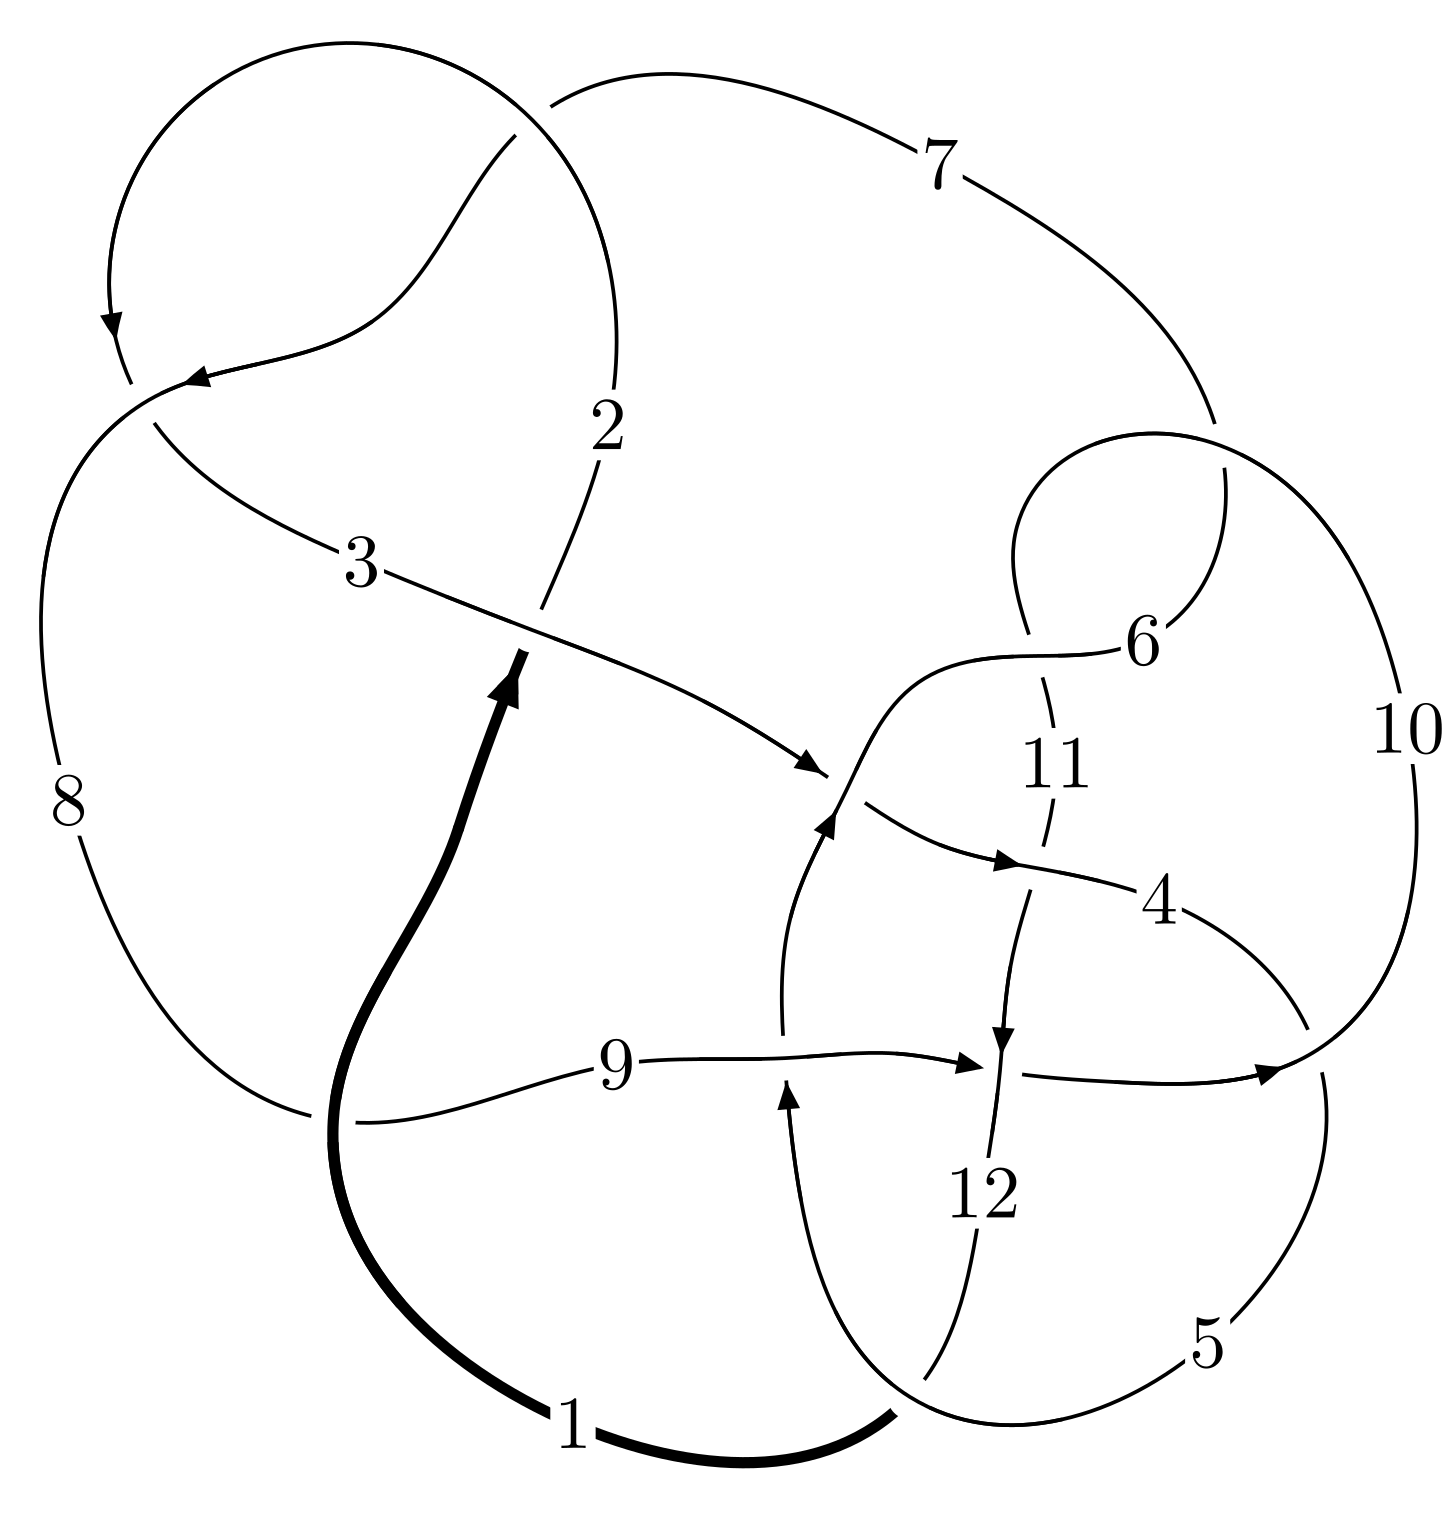
\includegraphics[width=112pt]{../../../GIT/diagram.site/Diagrams/png/2702_12n_0613.png}\\
\ \ \ A knot diagram\footnotemark}&
\allowdisplaybreaks
\textbf{Linearized knot diagam} \\
\cline{2-2}
 &
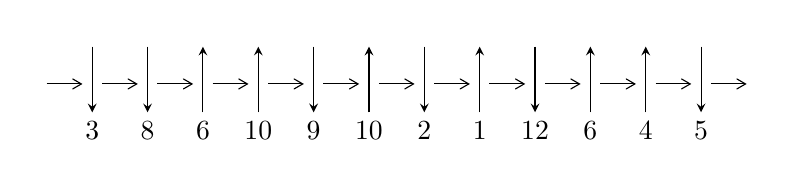
\begin{tikzpicture}[x=20pt, y=17pt]
	% nodes
	\node (C0) at (0, 0) {};
	\node (C1) at (1, 0) {};
	\node (C1U) at (1, +1) {};
	\node (C1D) at (1, -1) {3};

	\node (C2) at (2, 0) {};
	\node (C2U) at (2, +1) {};
	\node (C2D) at (2, -1) {8};

	\node (C3) at (3, 0) {};
	\node (C3U) at (3, +1) {};
	\node (C3D) at (3, -1) {6};

	\node (C4) at (4, 0) {};
	\node (C4U) at (4, +1) {};
	\node (C4D) at (4, -1) {10};

	\node (C5) at (5, 0) {};
	\node (C5U) at (5, +1) {};
	\node (C5D) at (5, -1) {9};

	\node (C6) at (6, 0) {};
	\node (C6U) at (6, +1) {};
	\node (C6D) at (6, -1) {10};

	\node (C7) at (7, 0) {};
	\node (C7U) at (7, +1) {};
	\node (C7D) at (7, -1) {2};

	\node (C8) at (8, 0) {};
	\node (C8U) at (8, +1) {};
	\node (C8D) at (8, -1) {1};

	\node (C9) at (9, 0) {};
	\node (C9U) at (9, +1) {};
	\node (C9D) at (9, -1) {12};

	\node (C10) at (10, 0) {};
	\node (C10U) at (10, +1) {};
	\node (C10D) at (10, -1) {6};

	\node (C11) at (11, 0) {};
	\node (C11U) at (11, +1) {};
	\node (C11D) at (11, -1) {4};

	\node (C12) at (12, 0) {};
	\node (C12U) at (12, +1) {};
	\node (C12D) at (12, -1) {5};
	\node (C13) at (13, 0) {};

	% arrows
	\draw[->,>={angle 60}]
	(C0) edge (C1) (C1) edge (C2) (C2) edge (C3) (C3) edge (C4) (C4) edge (C5) (C5) edge (C6) (C6) edge (C7) (C7) edge (C8) (C8) edge (C9) (C9) edge (C10) (C10) edge (C11) (C11) edge (C12) (C12) edge (C13) ;	\draw[->,>=stealth]
	(C1U) edge (C1D) (C2U) edge (C2D) (C3D) edge (C3U) (C4D) edge (C4U) (C5U) edge (C5D) (C6D) edge (C6U) (C7U) edge (C7D) (C8D) edge (C8U) (C9U) edge (C9D) (C10D) edge (C10U) (C11D) edge (C11U) (C12U) edge (C12D) ;
	\end{tikzpicture} \\
\hhline{~~} \\& 
\textbf{Solving Sequence} \\ \cline{2-2} 
 &
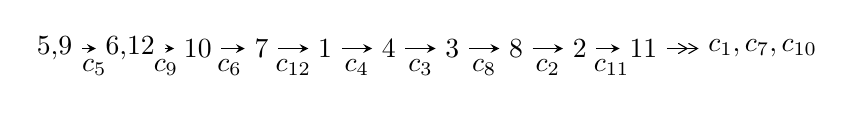
\begin{tikzpicture}[x=23pt, y=7pt]
	% node
	\node (A0) at (-1/8, 0) {5,9};
	\node (A1) at (17/16, 0) {6,12};
	\node (A2) at (17/8, 0) {10};
	\node (A3) at (25/8, 0) {7};
	\node (A4) at (33/8, 0) {1};
	\node (A5) at (41/8, 0) {4};
	\node (A6) at (49/8, 0) {3};
	\node (A7) at (57/8, 0) {8};
	\node (A8) at (65/8, 0) {2};
	\node (A9) at (73/8, 0) {11};
	\node (C1) at (1/2, -1) {$c_{5}$};
	\node (C2) at (13/8, -1) {$c_{9}$};
	\node (C3) at (21/8, -1) {$c_{6}$};
	\node (C4) at (29/8, -1) {$c_{12}$};
	\node (C5) at (37/8, -1) {$c_{4}$};
	\node (C6) at (45/8, -1) {$c_{3}$};
	\node (C7) at (53/8, -1) {$c_{8}$};
	\node (C8) at (61/8, -1) {$c_{2}$};
	\node (C9) at (69/8, -1) {$c_{11}$};
	\node (A10) at (11, 0) {$c_{1},c_{7},c_{10}$};

	% edge
	\draw[->,>=stealth]	
	(A0) edge (A1) (A1) edge (A2) (A2) edge (A3) (A3) edge (A4) (A4) edge (A5) (A5) edge (A6) (A6) edge (A7) (A7) edge (A8) (A8) edge (A9) ;
	\draw[->>,>={angle 60}]	
	(A9) edge (A10);
\end{tikzpicture} \\ 

\end{tabular} \\

\footnotetext{
The image of knot diagram is generated by the software ``\textbf{Draw programme}" developed by Andrew Bartholomew(\url{http://www.layer8.co.uk/maths/draw/index.htm\#Running-draw}), where we modified some parts for our purpose(\url{https://github.com/CATsTAILs/LinksPainter}).
}\phantom \\ \newline 
\centering \textbf{Ideals for irreducible components\footnotemark of $X_{\text{par}}$} 
 
\begin{align*}
I^u_{1}&=\langle 
b- u,\;5.43932\times10^{30} u^{31}+8.12908\times10^{30} u^{30}+\cdots+3.35339\times10^{30} a-9.00124\times10^{30},\\
\phantom{I^u_{1}}&\phantom{= \langle  }u^{32}+u^{31}+\cdots-5 u+1\rangle \\
I^u_{2}&=\langle 
b+u,\;-2006601310117 u^{21}-1475756618264 u^{20}+\cdots+214817393669 a-6503947392620,\\
\phantom{I^u_{2}}&\phantom{= \langle  }u^{22}+u^{21}+\cdots+6 u+1\rangle \\
I^u_{3}&=\langle 
2.83028\times10^{140} u^{47}+8.71962\times10^{140} u^{46}+\cdots+1.13769\times10^{141} b-1.39265\times10^{141},\\
\phantom{I^u_{3}}&\phantom{= \langle  }6.79051\times10^{120} u^{47}+2.06789\times10^{121} u^{46}+\cdots+6.50621\times10^{120} a-3.02432\times10^{121},\;u^{48}+3 u^{47}+\cdots-14 u+1\rangle \\
\\
\end{align*}
\raggedright * 3 irreducible components of $\dim_{\mathbb{C}}=0$, with total 102 representations.\\
\footnotetext{All coefficients of polynomials are rational numbers. But the coefficients are sometimes approximated in decimal forms when there is not enough margin.}
\newpage
\renewcommand{\arraystretch}{1}
\centering \section*{I. $I^u_{1}= \langle b- u,\;5.44\times10^{30} u^{31}+8.13\times10^{30} u^{30}+\cdots+3.35\times10^{30} a-9.00\times10^{30},\;u^{32}+u^{31}+\cdots-5 u+1 \rangle$}
\flushleft \textbf{(i) Arc colorings}\\
\begin{tabular}{m{7pt} m{180pt} m{7pt} m{180pt} }
\flushright $a_{5}=$&$\begin{pmatrix}1\\0\end{pmatrix}$ \\
\flushright $a_{9}=$&$\begin{pmatrix}0\\u\end{pmatrix}$ \\
\flushright $a_{6}=$&$\begin{pmatrix}1\\u^2\end{pmatrix}$ \\
\flushright $a_{12}=$&$\begin{pmatrix}-1.62204 u^{31}-2.42414 u^{30}+\cdots-16.2084 u+2.68422\\u\end{pmatrix}$ \\
\flushright $a_{10}=$&$\begin{pmatrix}-5.53414 u^{31}-6.62833 u^{30}+\cdots-35.0052 u+20.9674\\0.249234 u^{31}+0.273240 u^{30}+\cdots+3.38846 u-0.802100\end{pmatrix}$ \\
\flushright $a_{7}=$&$\begin{pmatrix}-7.19778 u^{31}-9.20184 u^{30}+\cdots-52.2087 u+21.0419\\0.101749 u^{31}+0.189658 u^{30}+\cdots+1.30173 u+0.191010\end{pmatrix}$ \\
\flushright $a_{1}=$&$\begin{pmatrix}-1.62204 u^{31}-2.42414 u^{30}+\cdots-17.2084 u+2.68422\\u\end{pmatrix}$ \\
\flushright $a_{4}=$&$\begin{pmatrix}0.441611 u^{31}+0.993111 u^{30}+\cdots+10.9819 u+4.63637\\0.0376695 u^{31}+0.0100421 u^{30}+\cdots+1.01416 u-0.742510\end{pmatrix}$ \\
\flushright $a_{3}=$&$\begin{pmatrix}0.543360 u^{31}+1.18277 u^{30}+\cdots+12.2837 u+4.82738\\0.0198247 u^{31}-0.00142549 u^{30}+\cdots+1.35196 u-0.830419\end{pmatrix}$ \\
\flushright $a_{8}=$&$\begin{pmatrix}-6.03260 u^{31}-7.17481 u^{30}+\cdots-39.7822 u+22.5716\\0.249234 u^{31}+0.273240 u^{30}+\cdots+3.38846 u-0.802100\end{pmatrix}$ \\
\flushright $a_{2}=$&$\begin{pmatrix}-8.35596 u^{31}-10.3141 u^{30}+\cdots-49.1564 u+32.2862\\0.207248 u^{31}+0.365116 u^{30}+\cdots+2.95393 u-0.843951\end{pmatrix}$ \\
\flushright $a_{11}=$&$\begin{pmatrix}-5.04086 u^{31}-6.12139 u^{30}+\cdots-31.6800 u+19.0711\\0.257866 u^{31}+0.306994 u^{30}+\cdots+2.96350 u-0.815763\end{pmatrix}$\\&\end{tabular}
\flushleft \textbf{(ii) Obstruction class $= -1$}\\~\\
\flushleft \textbf{(iii) Cusp Shapes $= 7.99213 u^{31}+9.89259 u^{30}+\cdots+52.3956 u-21.8422$}\\~\\
\newpage\renewcommand{\arraystretch}{1}
\flushleft \textbf{(iv) u-Polynomials at the component}\newline \\
\begin{tabular}{m{50pt}|m{274pt}}
Crossings & \hspace{64pt}u-Polynomials at each crossing \\
\hline $$\begin{aligned}c_{1}\end{aligned}$$&$\begin{aligned}
&u^{32}+16 u^{31}+\cdots-384 u+256
\end{aligned}$\\
\hline $$\begin{aligned}c_{2},c_{7}\end{aligned}$$&$\begin{aligned}
&u^{32}-8 u^{31}+\cdots-128 u+16
\end{aligned}$\\
\hline $$\begin{aligned}c_{3}\end{aligned}$$&$\begin{aligned}
&u^{32}+22 u^{31}+\cdots+27648 u+4096
\end{aligned}$\\
\hline $$\begin{aligned}c_{4}\end{aligned}$$&$\begin{aligned}
&u^{32}-8 u^{30}+\cdots+7 u-6
\end{aligned}$\\
\hline $$\begin{aligned}c_{5},c_{12}\end{aligned}$$&$\begin{aligned}
&u^{32}+u^{31}+\cdots-5 u+1
\end{aligned}$\\
\hline $$\begin{aligned}c_{6},c_{10},c_{11}\end{aligned}$$&$\begin{aligned}
&u^{32}-23 u^{30}+\cdots-9 u^2+1
\end{aligned}$\\
\hline $$\begin{aligned}c_{8}\end{aligned}$$&$\begin{aligned}
&u^{32}-24 u^{31}+\cdots-24064 u-2544
\end{aligned}$\\
\hline $$\begin{aligned}c_{9}\end{aligned}$$&$\begin{aligned}
&u^{32}-21 u^{31}+\cdots-992 u+64
\end{aligned}$\\
\hline
\end{tabular}\\~\\
\newpage\renewcommand{\arraystretch}{1}
\flushleft \textbf{(v) Riley Polynomials at the component}\newline \\
\begin{tabular}{m{50pt}|m{274pt}}
Crossings & \hspace{64pt}Riley Polynomials at each crossing \\
\hline $$\begin{aligned}c_{1}\end{aligned}$$&$\begin{aligned}
&y^{32}+4 y^{31}+\cdots-614400 y+65536
\end{aligned}$\\
\hline $$\begin{aligned}c_{2},c_{7}\end{aligned}$$&$\begin{aligned}
&y^{32}-16 y^{31}+\cdots+384 y+256
\end{aligned}$\\
\hline $$\begin{aligned}c_{3}\end{aligned}$$&$\begin{aligned}
&y^{32}-30 y^{31}+\cdots-131072000 y+16777216
\end{aligned}$\\
\hline $$\begin{aligned}c_{4}\end{aligned}$$&$\begin{aligned}
&y^{32}-16 y^{31}+\cdots-661 y+36
\end{aligned}$\\
\hline $$\begin{aligned}c_{5},c_{12}\end{aligned}$$&$\begin{aligned}
&y^{32}+3 y^{31}+\cdots-11 y+1
\end{aligned}$\\
\hline $$\begin{aligned}c_{6},c_{10},c_{11}\end{aligned}$$&$\begin{aligned}
&y^{32}-46 y^{31}+\cdots-18 y+1
\end{aligned}$\\
\hline $$\begin{aligned}c_{8}\end{aligned}$$&$\begin{aligned}
&y^{32}+14 y^{31}+\cdots-3117275776 y+6471936
\end{aligned}$\\
\hline $$\begin{aligned}c_{9}\end{aligned}$$&$\begin{aligned}
&y^{32}+9 y^{31}+\cdots+39936 y+4096
\end{aligned}$\\
\hline
\end{tabular}\\~\\
\newpage\flushleft \textbf{(vi) Complex Volumes and Cusp Shapes}
$$\begin{array}{c|c|c}  
\text{Solutions to }I^u_{1}& \I (\text{vol} + \sqrt{-1}CS) & \text{Cusp shape}\\
 \hline 
\begin{aligned}
u &= -0.390564 + 0.967977 I \\
a &= -1.60621 - 0.49572 I \\
b &= -0.390564 + 0.967977 I\end{aligned}
 & \phantom{-}9.63313 + 1.78314 I & \phantom{-}5.24416 - 2.15129 I \\ \hline\begin{aligned}
u &= -0.390564 - 0.967977 I \\
a &= -1.60621 + 0.49572 I \\
b &= -0.390564 - 0.967977 I\end{aligned}
 & \phantom{-}9.63313 - 1.78314 I & \phantom{-}5.24416 + 2.15129 I \\ \hline\begin{aligned}
u &= -0.859015 + 0.595187 I \\
a &= -0.70225 - 1.35017 I \\
b &= -0.859015 + 0.595187 I\end{aligned}
 & \phantom{-}3.11013 + 9.06642 I & -0.91274 - 7.85173 I \\ \hline\begin{aligned}
u &= -0.859015 - 0.595187 I \\
a &= -0.70225 + 1.35017 I \\
b &= -0.859015 - 0.595187 I\end{aligned}
 & \phantom{-}3.11013 - 9.06642 I & -0.91274 + 7.85173 I \\ \hline\begin{aligned}
u &= -0.519398 + 0.932460 I \\
a &= -0.647989 - 0.004890 I \\
b &= -0.519398 + 0.932460 I\end{aligned}
 & \phantom{-}1.88830 + 3.18747 I & \phantom{-}4.96056 - 5.55794 I \\ \hline\begin{aligned}
u &= -0.519398 - 0.932460 I \\
a &= -0.647989 + 0.004890 I \\
b &= -0.519398 - 0.932460 I\end{aligned}
 & \phantom{-}1.88830 - 3.18747 I & \phantom{-}4.96056 + 5.55794 I \\ \hline\begin{aligned}
u &= \phantom{-}0.275358 + 0.858528 I \\
a &= \phantom{-}0.738399 - 0.042001 I \\
b &= \phantom{-}0.275358 + 0.858528 I\end{aligned}
 & \phantom{-}2.15595 + 1.03231 I & \phantom{-}4.92013 - 2.65648 I \\ \hline\begin{aligned}
u &= \phantom{-}0.275358 - 0.858528 I \\
a &= \phantom{-}0.738399 + 0.042001 I \\
b &= \phantom{-}0.275358 - 0.858528 I\end{aligned}
 & \phantom{-}2.15595 - 1.03231 I & \phantom{-}4.92013 + 2.65648 I \\ \hline\begin{aligned}
u &= \phantom{-}0.657277 + 0.519284 I \\
a &= \phantom{-}0.91075 - 1.90121 I \\
b &= \phantom{-}0.657277 + 0.519284 I\end{aligned}
 & \phantom{-}5.54728 - 3.21063 I & \phantom{-}1.80460 + 6.59174 I \\ \hline\begin{aligned}
u &= \phantom{-}0.657277 - 0.519284 I \\
a &= \phantom{-}0.91075 + 1.90121 I \\
b &= \phantom{-}0.657277 - 0.519284 I\end{aligned}
 & \phantom{-}5.54728 + 3.21063 I & \phantom{-}1.80460 - 6.59174 I\\
 \hline 
 \end{array}$$\newpage$$\begin{array}{c|c|c}  
\text{Solutions to }I^u_{1}& \I (\text{vol} + \sqrt{-1}CS) & \text{Cusp shape}\\
 \hline 
\begin{aligned}
u &= -0.791811\phantom{ +0.000000I} \\
a &= -1.98040\phantom{ +0.000000I} \\
b &= -0.791811\phantom{ +0.000000I}\end{aligned}
 & -1.01617\phantom{ +0.000000I} & -9.04870\phantom{ +0.000000I} \\ \hline\begin{aligned}
u &= -0.755035\phantom{ +0.000000I} \\
a &= -0.694813\phantom{ +0.000000I} \\
b &= -0.755035\phantom{ +0.000000I}\end{aligned}
 & -1.77548\phantom{ +0.000000I} & -4.53550\phantom{ +0.000000I} \\ \hline\begin{aligned}
u &= \phantom{-}0.621825 + 1.097920 I \\
a &= \phantom{-}1.294920 - 0.198954 I \\
b &= \phantom{-}0.621825 + 1.097920 I\end{aligned}
 & \phantom{-}9.99995 - 7.71025 I & \phantom{-}4.49240 + 6.45370 I \\ \hline\begin{aligned}
u &= \phantom{-}0.621825 - 1.097920 I \\
a &= \phantom{-}1.294920 + 0.198954 I \\
b &= \phantom{-}0.621825 - 1.097920 I\end{aligned}
 & \phantom{-}9.99995 + 7.71025 I & \phantom{-}4.49240 - 6.45370 I \\ \hline\begin{aligned}
u &= \phantom{-}0.313313 + 0.638057 I \\
a &= -1.166610 - 0.622327 I \\
b &= \phantom{-}0.313313 + 0.638057 I\end{aligned}
 & -2.47132 - 5.60513 I & -2.05099 + 8.20859 I \\ \hline\begin{aligned}
u &= \phantom{-}0.313313 - 0.638057 I \\
a &= -1.166610 + 0.622327 I \\
b &= \phantom{-}0.313313 - 0.638057 I\end{aligned}
 & -2.47132 + 5.60513 I & -2.05099 - 8.20859 I \\ \hline\begin{aligned}
u &= -0.956018 + 0.923610 I \\
a &= -0.573225 + 0.070285 I \\
b &= -0.956018 + 0.923610 I\end{aligned}
 & -0.91090 + 3.64926 I & \phantom{-}4.33113 - 1.37429 I \\ \hline\begin{aligned}
u &= -0.956018 - 0.923610 I \\
a &= -0.573225 - 0.070285 I \\
b &= -0.956018 - 0.923610 I\end{aligned}
 & -0.91090 - 3.64926 I & \phantom{-}4.33113 + 1.37429 I \\ \hline\begin{aligned}
u &= \phantom{-}1.086610 + 0.795029 I \\
a &= \phantom{-}0.574623 + 0.109929 I \\
b &= \phantom{-}1.086610 + 0.795029 I\end{aligned}
 & -4.85287 + 0.14998 I & -1.49645 - 3.04413 I \\ \hline\begin{aligned}
u &= \phantom{-}1.086610 - 0.795029 I \\
a &= \phantom{-}0.574623 - 0.109929 I \\
b &= \phantom{-}1.086610 - 0.795029 I\end{aligned}
 & -4.85287 - 0.14998 I & -1.49645 + 3.04413 I\\
 \hline 
 \end{array}$$\newpage$$\begin{array}{c|c|c}  
\text{Solutions to }I^u_{1}& \I (\text{vol} + \sqrt{-1}CS) & \text{Cusp shape}\\
 \hline 
\begin{aligned}
u &= -1.06617 + 0.94422 I \\
a &= -1.051680 + 0.248881 I \\
b &= -1.06617 + 0.94422 I\end{aligned}
 & \phantom{-}1.89136 + 7.99794 I & -1.89042 - 4.55066 I \\ \hline\begin{aligned}
u &= -1.06617 - 0.94422 I \\
a &= -1.051680 - 0.248881 I \\
b &= -1.06617 - 0.94422 I\end{aligned}
 & \phantom{-}1.89136 - 7.99794 I & -1.89042 + 4.55066 I \\ \hline\begin{aligned}
u &= -0.075680 + 0.568202 I \\
a &= \phantom{-}1.265330 - 0.049232 I \\
b &= -0.075680 + 0.568202 I\end{aligned}
 & \phantom{-}0.51553 + 1.38561 I & \phantom{-}2.36633 - 4.82018 I \\ \hline\begin{aligned}
u &= -0.075680 - 0.568202 I \\
a &= \phantom{-}1.265330 + 0.049232 I \\
b &= -0.075680 - 0.568202 I\end{aligned}
 & \phantom{-}0.51553 - 1.38561 I & \phantom{-}2.36633 + 4.82018 I \\ \hline\begin{aligned}
u &= \phantom{-}1.03468 + 1.01787 I \\
a &= \phantom{-}0.546848 + 0.069159 I \\
b &= \phantom{-}1.03468 + 1.01787 I\end{aligned}
 & -3.90029 - 8.39051 I & \phantom{-}2.20035 + 3.96164 I \\ \hline\begin{aligned}
u &= \phantom{-}1.03468 - 1.01787 I \\
a &= \phantom{-}0.546848 - 0.069159 I \\
b &= \phantom{-}1.03468 - 1.01787 I\end{aligned}
 & -3.90029 + 8.39051 I & \phantom{-}2.20035 - 3.96164 I \\ \hline\begin{aligned}
u &= \phantom{-}1.09517 + 1.16567 I \\
a &= \phantom{-}0.950401 + 0.099835 I \\
b &= \phantom{-}1.09517 + 1.16567 I\end{aligned}
 & \phantom{-}7.31268 - 11.42420 I & \phantom{-0.000000 } 0 \\ \hline\begin{aligned}
u &= \phantom{-}1.09517 - 1.16567 I \\
a &= \phantom{-}0.950401 - 0.099835 I \\
b &= \phantom{-}1.09517 - 1.16567 I\end{aligned}
 & \phantom{-}7.31268 + 11.42420 I & \phantom{-0.000000 } 0 \\ \hline\begin{aligned}
u &= -1.21195 + 1.18977 I \\
a &= -0.876418 + 0.125795 I \\
b &= -1.21195 + 1.18977 I\end{aligned}
 & \phantom{-}4.7481 + 16.9486 I & \phantom{-0.000000 } 0 \\ \hline\begin{aligned}
u &= -1.21195 - 1.18977 I \\
a &= -0.876418 - 0.125795 I \\
b &= -1.21195 - 1.18977 I\end{aligned}
 & \phantom{-}4.7481 - 16.9486 I & \phantom{-0.000000 } 0\\
 \hline 
 \end{array}$$\newpage$$\begin{array}{c|c|c}  
\text{Solutions to }I^u_{1}& \I (\text{vol} + \sqrt{-1}CS) & \text{Cusp shape}\\
 \hline 
\begin{aligned}
u &= \phantom{-}0.267983 + 0.096022 I \\
a &= -3.81929 - 5.94198 I \\
b &= \phantom{-}0.267983 + 0.096022 I\end{aligned}
 & -2.01749 + 2.84138 I & -3.8195 + 16.5875 I \\ \hline\begin{aligned}
u &= \phantom{-}0.267983 - 0.096022 I \\
a &= -3.81929 + 5.94198 I \\
b &= \phantom{-}0.267983 - 0.096022 I\end{aligned}
 & -2.01749 - 2.84138 I & -3.8195 - 16.5875 I\\
 \hline 
 \end{array}$$\newpage\newpage\renewcommand{\arraystretch}{1}
\centering \section*{II. $I^u_{2}= \langle b+u,\;-2.01\times10^{12} u^{21}-1.48\times10^{12} u^{20}+\cdots+2.15\times10^{11} a-6.50\times10^{12},\;u^{22}+u^{21}+\cdots+6 u+1 \rangle$}
\flushleft \textbf{(i) Arc colorings}\\
\begin{tabular}{m{7pt} m{180pt} m{7pt} m{180pt} }
\flushright $a_{5}=$&$\begin{pmatrix}1\\0\end{pmatrix}$ \\
\flushright $a_{9}=$&$\begin{pmatrix}0\\u\end{pmatrix}$ \\
\flushright $a_{6}=$&$\begin{pmatrix}1\\u^2\end{pmatrix}$ \\
\flushright $a_{12}=$&$\begin{pmatrix}9.34096 u^{21}+6.86982 u^{20}+\cdots+89.6739 u+30.2766\\- u\end{pmatrix}$ \\
\flushright $a_{10}=$&$\begin{pmatrix}14.5794 u^{21}+8.87809 u^{20}+\cdots+142.535 u+28.7075\\0.590428 u^{21}+0.491225 u^{20}+\cdots+6.48590 u+2.47114\end{pmatrix}$ \\
\flushright $a_{7}=$&$\begin{pmatrix}-30.2766 u^{21}-20.9357 u^{20}+\cdots-297.306 u-90.9859\\-0.439803 u^{21}-0.428977 u^{20}+\cdots-4.50594 u-2.28936\end{pmatrix}$ \\
\flushright $a_{1}=$&$\begin{pmatrix}9.34096 u^{21}+6.86982 u^{20}+\cdots+90.6739 u+30.2766\\- u\end{pmatrix}$ \\
\flushright $a_{4}=$&$\begin{pmatrix}-8.47114 u^{21}-6.88072 u^{20}+\cdots-81.7691 u-36.3410\\0.340599 u^{21}+0.259687 u^{20}+\cdots+3.43451 u+0.698927\end{pmatrix}$ \\
\flushright $a_{3}=$&$\begin{pmatrix}-8.91095 u^{21}-7.30969 u^{20}+\cdots-86.2751 u-38.6303\\0.499053 u^{21}+0.260079 u^{20}+\cdots+3.80936 u+0.688101\end{pmatrix}$ \\
\flushright $a_{8}=$&$\begin{pmatrix}13.3986 u^{21}+7.89564 u^{20}+\cdots+131.564 u+23.7653\\0.590428 u^{21}+0.491225 u^{20}+\cdots+6.48590 u+2.47114\end{pmatrix}$ \\
\flushright $a_{2}=$&$\begin{pmatrix}20.5604 u^{21}+11.9205 u^{20}+\cdots+201.038 u+37.4919\\1.44804 u^{21}+0.929665 u^{20}+\cdots+12.8961 u+4.26770\end{pmatrix}$ \\
\flushright $a_{11}=$&$\begin{pmatrix}13.2901 u^{21}+8.02853 u^{20}+\cdots+129.393 u+25.4774\\0.579602 u^{21}+0.321944 u^{20}+\cdots+5.13644 u+2.03134\end{pmatrix}$\\&\end{tabular}
\flushleft \textbf{(ii) Obstruction class $= 1$}\\~\\
\flushleft \textbf{(iii) Cusp Shapes $= -\frac{8090826551153}{214817393669} u^{21}-\frac{5909957309789}{214817393669} u^{20}+\cdots-\frac{76582895018229}{214817393669} u-\frac{30531044823813}{214817393669}$}\\~\\
\newpage\renewcommand{\arraystretch}{1}
\flushleft \textbf{(iv) u-Polynomials at the component}\newline \\
\begin{tabular}{m{50pt}|m{274pt}}
Crossings & \hspace{64pt}u-Polynomials at each crossing \\
\hline $$\begin{aligned}c_{1}\end{aligned}$$&$\begin{aligned}
&u^{22}-13 u^{21}+\cdots-8 u+1
\end{aligned}$\\
\hline $$\begin{aligned}c_{2}\end{aligned}$$&$\begin{aligned}
&u^{22}+u^{21}+\cdots-4 u^2+1
\end{aligned}$\\
\hline $$\begin{aligned}c_{3}\end{aligned}$$&$\begin{aligned}
&u^{22}+15 u^{21}+\cdots+132 u+29
\end{aligned}$\\
\hline $$\begin{aligned}c_{4}\end{aligned}$$&$\begin{aligned}
&u^{22}-5 u^{20}+\cdots-19 u+13
\end{aligned}$\\
\hline $$\begin{aligned}c_{5},c_{12}\end{aligned}$$&$\begin{aligned}
&u^{22}+u^{21}+\cdots+6 u+1
\end{aligned}$\\
\hline $$\begin{aligned}c_{6},c_{11}\end{aligned}$$&$\begin{aligned}
&u^{22}-2 u^{21}+\cdots- u+1
\end{aligned}$\\
\hline $$\begin{aligned}c_{7}\end{aligned}$$&$\begin{aligned}
&u^{22}- u^{21}+\cdots-4 u^2+1
\end{aligned}$\\
\hline $$\begin{aligned}c_{8}\end{aligned}$$&$\begin{aligned}
&u^{22}-3 u^{21}+\cdots-8 u^2+1
\end{aligned}$\\
\hline $$\begin{aligned}c_{9}\end{aligned}$$&$\begin{aligned}
&u^{22}-10 u^{21}+\cdots+3 u^2+1
\end{aligned}$\\
\hline $$\begin{aligned}c_{10}\end{aligned}$$&$\begin{aligned}
&u^{22}+2 u^{21}+\cdots+u+1
\end{aligned}$\\
\hline
\end{tabular}\\~\\
\newpage\renewcommand{\arraystretch}{1}
\flushleft \textbf{(v) Riley Polynomials at the component}\newline \\
\begin{tabular}{m{50pt}|m{274pt}}
Crossings & \hspace{64pt}Riley Polynomials at each crossing \\
\hline $$\begin{aligned}c_{1}\end{aligned}$$&$\begin{aligned}
&y^{22}+3 y^{21}+\cdots-8 y+1
\end{aligned}$\\
\hline $$\begin{aligned}c_{2},c_{7}\end{aligned}$$&$\begin{aligned}
&y^{22}-13 y^{21}+\cdots-8 y+1
\end{aligned}$\\
\hline $$\begin{aligned}c_{3}\end{aligned}$$&$\begin{aligned}
&y^{22}-23 y^{21}+\cdots-7738 y+841
\end{aligned}$\\
\hline $$\begin{aligned}c_{4}\end{aligned}$$&$\begin{aligned}
&y^{22}-10 y^{21}+\cdots+1017 y+169
\end{aligned}$\\
\hline $$\begin{aligned}c_{5},c_{12}\end{aligned}$$&$\begin{aligned}
&y^{22}-7 y^{21}+\cdots-20 y+1
\end{aligned}$\\
\hline $$\begin{aligned}c_{6},c_{10},c_{11}\end{aligned}$$&$\begin{aligned}
&y^{22}-12 y^{21}+\cdots+17 y+1
\end{aligned}$\\
\hline $$\begin{aligned}c_{8}\end{aligned}$$&$\begin{aligned}
&y^{22}+13 y^{21}+\cdots-16 y+1
\end{aligned}$\\
\hline $$\begin{aligned}c_{9}\end{aligned}$$&$\begin{aligned}
&y^{22}+8 y^{21}+\cdots+6 y+1
\end{aligned}$\\
\hline
\end{tabular}\\~\\
\newpage\flushleft \textbf{(vi) Complex Volumes and Cusp Shapes}
$$\begin{array}{c|c|c}  
\text{Solutions to }I^u_{2}& \I (\text{vol} + \sqrt{-1}CS) & \text{Cusp shape}\\
 \hline 
\begin{aligned}
u &= -0.858443 + 0.472828 I \\
a &= -0.268594 - 0.545737 I \\
b &= \phantom{-}0.858443 - 0.472828 I\end{aligned}
 & \phantom{-}6.63217 - 1.18036 I & \phantom{-}3.98252 - 0.95830 I \\ \hline\begin{aligned}
u &= -0.858443 - 0.472828 I \\
a &= -0.268594 + 0.545737 I \\
b &= \phantom{-}0.858443 + 0.472828 I\end{aligned}
 & \phantom{-}6.63217 + 1.18036 I & \phantom{-}3.98252 + 0.95830 I \\ \hline\begin{aligned}
u &= -0.969570 + 0.104792 I \\
a &= \phantom{-}0.958370 - 1.015960 I \\
b &= \phantom{-}0.969570 - 0.104792 I\end{aligned}
 & -4.48502 + 5.07387 I & -8.63863 - 8.30587 I \\ \hline\begin{aligned}
u &= -0.969570 - 0.104792 I \\
a &= \phantom{-}0.958370 + 1.015960 I \\
b &= \phantom{-}0.969570 + 0.104792 I\end{aligned}
 & -4.48502 - 5.07387 I & -8.63863 + 8.30587 I \\ \hline\begin{aligned}
u &= -0.362670 + 0.880683 I \\
a &= \phantom{-}0.684664 - 0.540153 I \\
b &= \phantom{-}0.362670 - 0.880683 I\end{aligned}
 & \phantom{-}4.53253 - 2.07273 I & \phantom{-}8.32895 + 4.83845 I \\ \hline\begin{aligned}
u &= -0.362670 - 0.880683 I \\
a &= \phantom{-}0.684664 + 0.540153 I \\
b &= \phantom{-}0.362670 + 0.880683 I\end{aligned}
 & \phantom{-}4.53253 + 2.07273 I & \phantom{-}8.32895 - 4.83845 I \\ \hline\begin{aligned}
u &= \phantom{-}0.647068 + 0.985785 I \\
a &= -0.320022 - 0.399758 I \\
b &= -0.647068 - 0.985785 I\end{aligned}
 & \phantom{-}3.43411 - 0.50011 I & \phantom{-}2.53542 + 4.24945 I \\ \hline\begin{aligned}
u &= \phantom{-}0.647068 - 0.985785 I \\
a &= -0.320022 + 0.399758 I \\
b &= -0.647068 + 0.985785 I\end{aligned}
 & \phantom{-}3.43411 + 0.50011 I & \phantom{-}2.53542 - 4.24945 I \\ \hline\begin{aligned}
u &= \phantom{-}1.153990 + 0.411356 I \\
a &= -0.864989 - 0.491617 I \\
b &= -1.153990 - 0.411356 I\end{aligned}
 & -2.39449 - 2.98768 I & \phantom{-}1.98501 + 3.10922 I \\ \hline\begin{aligned}
u &= \phantom{-}1.153990 - 0.411356 I \\
a &= -0.864989 + 0.491617 I \\
b &= -1.153990 + 0.411356 I\end{aligned}
 & -2.39449 + 2.98768 I & \phantom{-}1.98501 - 3.10922 I\\
 \hline 
 \end{array}$$\newpage$$\begin{array}{c|c|c}  
\text{Solutions to }I^u_{2}& \I (\text{vol} + \sqrt{-1}CS) & \text{Cusp shape}\\
 \hline 
\begin{aligned}
u &= \phantom{-}1.027480 + 0.719532 I \\
a &= \phantom{-}0.048327 - 0.358842 I \\
b &= -1.027480 - 0.719532 I\end{aligned}
 & \phantom{-}4.91059 + 5.90541 I & \phantom{-}1.71844 - 3.95716 I \\ \hline\begin{aligned}
u &= \phantom{-}1.027480 - 0.719532 I \\
a &= \phantom{-}0.048327 + 0.358842 I \\
b &= -1.027480 + 0.719532 I\end{aligned}
 & \phantom{-}4.91059 - 5.90541 I & \phantom{-}1.71844 + 3.95716 I \\ \hline\begin{aligned}
u &= \phantom{-}0.470860 + 0.507733 I \\
a &= -2.04467 + 0.62131 I \\
b &= -0.470860 - 0.507733 I\end{aligned}
 & -0.39120 - 2.98356 I & -1.48889 + 12.19524 I \\ \hline\begin{aligned}
u &= \phantom{-}0.470860 - 0.507733 I \\
a &= -2.04467 - 0.62131 I \\
b &= -0.470860 + 0.507733 I\end{aligned}
 & -0.39120 + 2.98356 I & -1.48889 - 12.19524 I \\ \hline\begin{aligned}
u &= \phantom{-}1.015410 + 0.828466 I \\
a &= -0.835698 - 0.057216 I \\
b &= -1.015410 - 0.828466 I\end{aligned}
 & -1.82515 - 4.29426 I & -2.89416 + 5.12116 I \\ \hline\begin{aligned}
u &= \phantom{-}1.015410 - 0.828466 I \\
a &= -0.835698 + 0.057216 I \\
b &= -1.015410 + 0.828466 I\end{aligned}
 & -1.82515 + 4.29426 I & -2.89416 - 5.12116 I \\ \hline\begin{aligned}
u &= -1.23379 + 0.77502 I \\
a &= \phantom{-}0.728855 - 0.197315 I \\
b &= \phantom{-}1.23379 - 0.77502 I\end{aligned}
 & -5.39649 + 0.76944 I & -5.69205 - 1.85880 I \\ \hline\begin{aligned}
u &= -1.23379 - 0.77502 I \\
a &= \phantom{-}0.728855 + 0.197315 I \\
b &= \phantom{-}1.23379 + 0.77502 I\end{aligned}
 & -5.39649 - 0.76944 I & -5.69205 + 1.85880 I \\ \hline\begin{aligned}
u &= -1.08883 + 0.97192 I \\
a &= \phantom{-}0.712895 - 0.033605 I \\
b &= \phantom{-}1.08883 - 0.97192 I\end{aligned}
 & -4.58982 + 8.86717 I & -6.46501 - 9.30335 I \\ \hline\begin{aligned}
u &= -1.08883 - 0.97192 I \\
a &= \phantom{-}0.712895 + 0.033605 I \\
b &= \phantom{-}1.08883 + 0.97192 I\end{aligned}
 & -4.58982 - 8.86717 I & -6.46501 + 9.30335 I\\
 \hline 
 \end{array}$$\newpage$$\begin{array}{c|c|c}  
\text{Solutions to }I^u_{2}& \I (\text{vol} + \sqrt{-1}CS) & \text{Cusp shape}\\
 \hline 
\begin{aligned}
u &= -0.301500 + 0.088234 I \\
a &= \phantom{-}1.20086 + 7.48943 I \\
b &= \phantom{-}0.301500 - 0.088234 I\end{aligned}
 & -2.07217 + 2.98695 I & -23.8716 - 31.2516 I \\ \hline\begin{aligned}
u &= -0.301500 - 0.088234 I \\
a &= \phantom{-}1.20086 - 7.48943 I \\
b &= \phantom{-}0.301500 + 0.088234 I\end{aligned}
 & -2.07217 - 2.98695 I & -23.8716 + 31.2516 I\\
 \hline 
 \end{array}$$\newpage\newpage\renewcommand{\arraystretch}{1}
\centering \section*{III. $I^u_{3}= \langle 2.83\times10^{140} u^{47}+8.72\times10^{140} u^{46}+\cdots+1.14\times10^{141} b-1.39\times10^{141},\;6.79\times10^{120} u^{47}+2.07\times10^{121} u^{46}+\cdots+6.51\times10^{120} a-3.02\times10^{121},\;u^{48}+3 u^{47}+\cdots-14 u+1 \rangle$}
\flushleft \textbf{(i) Arc colorings}\\
\begin{tabular}{m{7pt} m{180pt} m{7pt} m{180pt} }
\flushright $a_{5}=$&$\begin{pmatrix}1\\0\end{pmatrix}$ \\
\flushright $a_{9}=$&$\begin{pmatrix}0\\u\end{pmatrix}$ \\
\flushright $a_{6}=$&$\begin{pmatrix}1\\u^2\end{pmatrix}$ \\
\flushright $a_{12}=$&$\begin{pmatrix}-1.04370 u^{47}-3.17834 u^{46}+\cdots-112.473 u+4.64836\\-0.248774 u^{47}-0.766430 u^{46}+\cdots-25.7903 u+1.22410\end{pmatrix}$ \\
\flushright $a_{10}=$&$\begin{pmatrix}0.352601 u^{47}+1.15475 u^{46}+\cdots+9.77743 u+5.15330\\0.0884410 u^{47}+0.277756 u^{46}+\cdots+5.39711 u+0.961781\end{pmatrix}$ \\
\flushright $a_{7}=$&$\begin{pmatrix}-0.459789 u^{47}-1.51384 u^{46}+\cdots-18.0243 u-5.98347\\-0.181840 u^{47}-0.582355 u^{46}+\cdots-10.3425 u-1.14025\end{pmatrix}$ \\
\flushright $a_{1}=$&$\begin{pmatrix}-0.794923 u^{47}-2.41191 u^{46}+\cdots-86.6830 u+3.42426\\-0.248774 u^{47}-0.766430 u^{46}+\cdots-25.7903 u+1.22410\end{pmatrix}$ \\
\flushright $a_{4}=$&$\begin{pmatrix}0.641629 u^{47}+2.09620 u^{46}+\cdots+28.3668 u+7.12371\\0.188784 u^{47}+0.597549 u^{46}+\cdots+12.0992 u+0.968939\end{pmatrix}$ \\
\flushright $a_{3}=$&$\begin{pmatrix}0.459789 u^{47}+1.51384 u^{46}+\cdots+18.0243 u+5.98347\\0.184999 u^{47}+0.586827 u^{46}+\cdots+11.7654 u+1.00577\end{pmatrix}$ \\
\flushright $a_{8}=$&$\begin{pmatrix}0.182173 u^{47}+0.616405 u^{46}+\cdots+2.12767 u+3.43309\\0.0819875 u^{47}+0.260591 u^{46}+\cdots+4.25265 u+0.758426\end{pmatrix}$ \\
\flushright $a_{2}=$&$\begin{pmatrix}0.182173 u^{47}+0.616405 u^{46}+\cdots+2.12767 u+3.43309\\0.0524818 u^{47}+0.165721 u^{46}+\cdots+2.21890 u+0.634265\end{pmatrix}$ \\
\flushright $a_{11}=$&$\begin{pmatrix}0.442236 u^{47}+1.43983 u^{46}+\cdots+14.1699 u+6.21203\\0.0885446 u^{47}+0.276604 u^{46}+\cdots+5.53392 u+0.945606\end{pmatrix}$\\&\end{tabular}
\flushleft \textbf{(ii) Obstruction class $= -1$}\\~\\
\flushleft \textbf{(iii) Cusp Shapes $= -0.726576 u^{47}-2.21182 u^{46}+\cdots-75.1418 u+5.51596$}\\~\\
\newpage\renewcommand{\arraystretch}{1}
\flushleft \textbf{(iv) u-Polynomials at the component}\newline \\
\begin{tabular}{m{50pt}|m{274pt}}
Crossings & \hspace{64pt}u-Polynomials at each crossing \\
\hline $$\begin{aligned}c_{1},c_{8}\end{aligned}$$&$\begin{aligned}
&(u^6+3 u^5+5 u^4+4 u^3+2 u^2+u+1)^8
\end{aligned}$\\
\hline $$\begin{aligned}c_{2},c_{7}\end{aligned}$$&$\begin{aligned}
&(u^6+u^5- u^4-2 u^3+u+1)^8
\end{aligned}$\\
\hline $$\begin{aligned}c_{3}\end{aligned}$$&$\begin{aligned}
&(u^4-3 u^3+u^2+2 u+1)^{12}
\end{aligned}$\\
\hline $$\begin{aligned}c_{4}\end{aligned}$$&$\begin{aligned}
&u^{48}+u^{47}+\cdots+30108 u+22357
\end{aligned}$\\
\hline $$\begin{aligned}c_{5},c_{12}\end{aligned}$$&$\begin{aligned}
&u^{48}+3 u^{47}+\cdots-14 u+1
\end{aligned}$\\
\hline $$\begin{aligned}c_{6},c_{10},c_{11}\end{aligned}$$&$\begin{aligned}
&u^{48}+u^{47}+\cdots+76002 u+31907
\end{aligned}$\\
\hline $$\begin{aligned}c_{9}\end{aligned}$$&$\begin{aligned}
&(u^4+u^3+u^2+1)^{12}
\end{aligned}$\\
\hline
\end{tabular}\\~\\
\newpage\renewcommand{\arraystretch}{1}
\flushleft \textbf{(v) Riley Polynomials at the component}\newline \\
\begin{tabular}{m{50pt}|m{274pt}}
Crossings & \hspace{64pt}Riley Polynomials at each crossing \\
\hline $$\begin{aligned}c_{1},c_{8}\end{aligned}$$&$\begin{aligned}
&(y^6+y^5+5 y^4+6 y^2+3 y+1)^8
\end{aligned}$\\
\hline $$\begin{aligned}c_{2},c_{7}\end{aligned}$$&$\begin{aligned}
&(y^6-3 y^5+5 y^4-4 y^3+2 y^2- y+1)^8
\end{aligned}$\\
\hline $$\begin{aligned}c_{3}\end{aligned}$$&$\begin{aligned}
&(y^4-7 y^3+15 y^2-2 y+1)^{12}
\end{aligned}$\\
\hline $$\begin{aligned}c_{4}\end{aligned}$$&$\begin{aligned}
&y^{48}-21 y^{47}+\cdots-2279703318 y+499835449
\end{aligned}$\\
\hline $$\begin{aligned}c_{5},c_{12}\end{aligned}$$&$\begin{aligned}
&y^{48}-9 y^{47}+\cdots+44 y+1
\end{aligned}$\\
\hline $$\begin{aligned}c_{6},c_{10},c_{11}\end{aligned}$$&$\begin{aligned}
&y^{48}-45 y^{47}+\cdots-3001288400 y+1018056649
\end{aligned}$\\
\hline $$\begin{aligned}c_{9}\end{aligned}$$&$\begin{aligned}
&(y^4+y^3+3 y^2+2 y+1)^{12}
\end{aligned}$\\
\hline
\end{tabular}\\~\\
\newpage\flushleft \textbf{(vi) Complex Volumes and Cusp Shapes}
$$\begin{array}{c|c|c}  
\text{Solutions to }I^u_{3}& \I (\text{vol} + \sqrt{-1}CS) & \text{Cusp shape}\\
 \hline 
\begin{aligned}
u &= \phantom{-}0.629593 + 0.781806 I \\
a &= -1.239320 + 0.091509 I \\
b &= -1.12594 - 0.99017 I\end{aligned}
 & \phantom{-}0.03467 - 4.08827 I & \phantom{-}3.88998 + 3.35903 I \\ \hline\begin{aligned}
u &= \phantom{-}0.629593 - 0.781806 I \\
a &= -1.239320 - 0.091509 I \\
b &= -1.12594 + 0.99017 I\end{aligned}
 & \phantom{-}0.03467 + 4.08827 I & \phantom{-}3.88998 - 3.35903 I \\ \hline\begin{aligned}
u &= \phantom{-}0.330707 + 0.926113 I \\
a &= \phantom{-}0.810156 - 0.090576 I \\
b &= \phantom{-}1.69106 - 0.76622 I\end{aligned}
 & \phantom{-}7.03641 - 0.49080 I & \phantom{-}7.54346 + 4.11452 I \\ \hline\begin{aligned}
u &= \phantom{-}0.330707 - 0.926113 I \\
a &= \phantom{-}0.810156 + 0.090576 I \\
b &= \phantom{-}1.69106 + 0.76622 I\end{aligned}
 & \phantom{-}7.03641 + 0.49080 I & \phantom{-}7.54346 - 4.11452 I \\ \hline\begin{aligned}
u &= -1.069080 + 0.043286 I \\
a &= \phantom{-}0.761004 + 0.883218 I \\
b &= \phantom{-}1.023650 + 0.361469 I\end{aligned}
 & -3.74655 - 4.08827 I & -3.54346 + 3.35903 I \\ \hline\begin{aligned}
u &= -1.069080 - 0.043286 I \\
a &= \phantom{-}0.761004 - 0.883218 I \\
b &= \phantom{-}1.023650 - 0.361469 I\end{aligned}
 & -3.74655 + 4.08827 I & -3.54346 - 3.35903 I \\ \hline\begin{aligned}
u &= \phantom{-}1.023650 + 0.361469 I \\
a &= -1.019380 - 0.530277 I \\
b &= -1.069080 + 0.043286 I\end{aligned}
 & -3.74655 - 4.08827 I & -3.54346 + 3.35903 I \\ \hline\begin{aligned}
u &= \phantom{-}1.023650 - 0.361469 I \\
a &= -1.019380 + 0.530277 I \\
b &= -1.069080 - 0.043286 I\end{aligned}
 & -3.74655 + 4.08827 I & -3.54346 - 3.35903 I \\ \hline\begin{aligned}
u &= -1.091250 + 0.090133 I \\
a &= -0.266053 - 0.682083 I \\
b &= \phantom{-}0.011750 - 1.180710 I\end{aligned}
 & \phantom{-}3.25520 - 2.33941 I & \phantom{-}0.11002 + 5.70297 I \\ \hline\begin{aligned}
u &= -1.091250 - 0.090133 I \\
a &= -0.266053 + 0.682083 I \\
b &= \phantom{-}0.011750 + 1.180710 I\end{aligned}
 & \phantom{-}3.25520 + 2.33941 I & \phantom{-}0.11002 - 5.70297 I\\
 \hline 
 \end{array}$$\newpage$$\begin{array}{c|c|c}  
\text{Solutions to }I^u_{3}& \I (\text{vol} + \sqrt{-1}CS) & \text{Cusp shape}\\
 \hline 
\begin{aligned}
u &= -0.542828 + 0.716452 I \\
a &= \phantom{-}1.380360 + 0.143081 I \\
b &= \phantom{-}0.238962 - 0.272108 I\end{aligned}
 & \phantom{-}0.03467 + 2.23966 I & \phantom{-}3.88998 - 1.77057 I \\ \hline\begin{aligned}
u &= -0.542828 - 0.716452 I \\
a &= \phantom{-}1.380360 - 0.143081 I \\
b &= \phantom{-}0.238962 + 0.272108 I\end{aligned}
 & \phantom{-}0.03467 - 2.23966 I & \phantom{-}3.88998 + 1.77057 I \\ \hline\begin{aligned}
u &= -0.358866 + 1.095930 I \\
a &= -0.688574 - 0.095537 I \\
b &= -1.90461 - 0.46488 I\end{aligned}
 & \phantom{-}5.14581 - 4.27792 I & \phantom{-}3.82674 + 0.60183 I \\ \hline\begin{aligned}
u &= -0.358866 - 1.095930 I \\
a &= -0.688574 + 0.095537 I \\
b &= -1.90461 + 0.46488 I\end{aligned}
 & \phantom{-}5.14581 + 4.27792 I & \phantom{-}3.82674 - 0.60183 I \\ \hline\begin{aligned}
u &= \phantom{-}0.011750 + 1.180710 I \\
a &= -0.607068 - 0.304005 I \\
b &= -1.091250 - 0.090133 I\end{aligned}
 & \phantom{-}3.25520 + 2.33941 I & \phantom{-0.000000 } 0. - 5.70297 I \\ \hline\begin{aligned}
u &= \phantom{-}0.011750 - 1.180710 I \\
a &= -0.607068 + 0.304005 I \\
b &= -1.091250 + 0.090133 I\end{aligned}
 & \phantom{-}3.25520 - 2.33941 I & \phantom{-0.000000 -}0. + 5.70297 I \\ \hline\begin{aligned}
u &= -0.755849 + 0.949728 I \\
a &= \phantom{-}1.024450 + 0.081577 I \\
b &= \phantom{-}1.36656 - 1.07638 I\end{aligned}
 & -1.85594 + 8.85698 I & \phantom{-0.000000 } 0. - 8.07537 I \\ \hline\begin{aligned}
u &= -0.755849 - 0.949728 I \\
a &= \phantom{-}1.024450 - 0.081577 I \\
b &= \phantom{-}1.36656 + 1.07638 I\end{aligned}
 & -1.85594 - 8.85698 I & \phantom{-0.000000 -}0. + 8.07537 I \\ \hline\begin{aligned}
u &= -1.030050 + 0.657859 I \\
a &= \phantom{-}0.988705 - 0.253254 I \\
b &= \phantom{-}1.41741 - 0.53201 I\end{aligned}
 & -3.74655 + 2.23966 I & -3.54346 + 0. I\phantom{ +0.000000I} \\ \hline\begin{aligned}
u &= -1.030050 - 0.657859 I \\
a &= \phantom{-}0.988705 + 0.253254 I \\
b &= \phantom{-}1.41741 + 0.53201 I\end{aligned}
 & -3.74655 - 2.23966 I & -3.54346 + 0. I\phantom{ +0.000000I}\\
 \hline 
 \end{array}$$\newpage$$\begin{array}{c|c|c}  
\text{Solutions to }I^u_{3}& \I (\text{vol} + \sqrt{-1}CS) & \text{Cusp shape}\\
 \hline 
\begin{aligned}
u &= -0.167396 + 0.661515 I \\
a &= -0.98845 + 1.53779 I \\
b &= \phantom{-}0.414199 - 0.088722 I\end{aligned}
 & -1.85594 + 2.52906 I & \phantom{-}0.17326 - 2.94577 I \\ \hline\begin{aligned}
u &= -0.167396 - 0.661515 I \\
a &= -0.98845 - 1.53779 I \\
b &= \phantom{-}0.414199 + 0.088722 I\end{aligned}
 & -1.85594 - 2.52906 I & \phantom{-}0.17326 + 2.94577 I \\ \hline\begin{aligned}
u &= \phantom{-}0.388273 + 0.497540 I \\
a &= \phantom{-}1.242770 + 0.262742 I \\
b &= \phantom{-}1.39675 - 1.46025 I\end{aligned}
 & \phantom{-}7.03641 - 2.33941 I & \phantom{-}7.54346 + 5.70297 I \\ \hline\begin{aligned}
u &= \phantom{-}0.388273 - 0.497540 I \\
a &= \phantom{-}1.242770 - 0.262742 I \\
b &= \phantom{-}1.39675 + 1.46025 I\end{aligned}
 & \phantom{-}7.03641 + 2.33941 I & \phantom{-}7.54346 - 5.70297 I \\ \hline\begin{aligned}
u &= -0.490886 + 0.302457 I \\
a &= -1.174830 + 0.743568 I \\
b &= -1.32499 - 1.79381 I\end{aligned}
 & \phantom{-}5.14581 + 7.10813 I & \phantom{-}3.82674 - 10.41931 I \\ \hline\begin{aligned}
u &= -0.490886 - 0.302457 I \\
a &= -1.174830 - 0.743568 I \\
b &= -1.32499 + 1.79381 I\end{aligned}
 & \phantom{-}5.14581 - 7.10813 I & \phantom{-}3.82674 + 10.41931 I \\ \hline\begin{aligned}
u &= -1.12594 + 0.99017 I \\
a &= \phantom{-}0.827967 - 0.081233 I \\
b &= \phantom{-}0.629593 - 0.781806 I\end{aligned}
 & \phantom{-}0.03467 + 4.08827 I & \phantom{-0.000000 } 0 \\ \hline\begin{aligned}
u &= -1.12594 - 0.99017 I \\
a &= \phantom{-}0.827967 + 0.081233 I \\
b &= \phantom{-}0.629593 + 0.781806 I\end{aligned}
 & \phantom{-}0.03467 - 4.08827 I & \phantom{-0.000000 } 0 \\ \hline\begin{aligned}
u &= \phantom{-}1.41741 + 0.53201 I \\
a &= -0.738267 - 0.365826 I \\
b &= -1.030050 - 0.657859 I\end{aligned}
 & -3.74655 - 2.23966 I & \phantom{-0.000000 } 0 \\ \hline\begin{aligned}
u &= \phantom{-}1.41741 - 0.53201 I \\
a &= -0.738267 + 0.365826 I \\
b &= -1.030050 + 0.657859 I\end{aligned}
 & -3.74655 + 2.23966 I & \phantom{-0.000000 } 0\\
 \hline 
 \end{array}$$\newpage$$\begin{array}{c|c|c}  
\text{Solutions to }I^u_{3}& \I (\text{vol} + \sqrt{-1}CS) & \text{Cusp shape}\\
 \hline 
\begin{aligned}
u &= \phantom{-}0.414199 + 0.088722 I \\
a &= -1.51570 + 2.52480 I \\
b &= -0.167396 - 0.661515 I\end{aligned}
 & -1.85594 - 2.52906 I & \phantom{-}0.17326 + 2.94577 I \\ \hline\begin{aligned}
u &= \phantom{-}0.414199 - 0.088722 I \\
a &= -1.51570 - 2.52480 I \\
b &= -0.167396 + 0.661515 I\end{aligned}
 & -1.85594 + 2.52906 I & \phantom{-}0.17326 - 2.94577 I \\ \hline\begin{aligned}
u &= \phantom{-}0.238962 + 0.272108 I \\
a &= -3.44289 + 0.10691 I \\
b &= -0.542828 - 0.716452 I\end{aligned}
 & \phantom{-}0.03467 - 2.23966 I & \phantom{-}3.88998 + 1.77057 I \\ \hline\begin{aligned}
u &= \phantom{-}0.238962 - 0.272108 I \\
a &= -3.44289 - 0.10691 I \\
b &= -0.542828 + 0.716452 I\end{aligned}
 & \phantom{-}0.03467 + 2.23966 I & \phantom{-}3.88998 - 1.77057 I \\ \hline\begin{aligned}
u &= -0.61144 + 1.52100 I \\
a &= \phantom{-}0.327664 - 0.363021 I \\
b &= \phantom{-}0.0642708 - 0.0873744 I\end{aligned}
 & \phantom{-}3.25520 - 0.49080 I & \phantom{-0.000000 } 0 \\ \hline\begin{aligned}
u &= -0.61144 - 1.52100 I \\
a &= \phantom{-}0.327664 + 0.363021 I \\
b &= \phantom{-}0.0642708 + 0.0873744 I\end{aligned}
 & \phantom{-}3.25520 + 0.49080 I & \phantom{-0.000000 } 0 \\ \hline\begin{aligned}
u &= \phantom{-}1.36656 + 1.07638 I \\
a &= -0.708821 - 0.108545 I \\
b &= -0.755849 - 0.949728 I\end{aligned}
 & -1.85594 - 8.85698 I & \phantom{-0.000000 } 0 \\ \hline\begin{aligned}
u &= \phantom{-}1.36656 - 1.07638 I \\
a &= -0.708821 + 0.108545 I \\
b &= -0.755849 + 0.949728 I\end{aligned}
 & -1.85594 + 8.85698 I & \phantom{-0.000000 } 0 \\ \hline\begin{aligned}
u &= \phantom{-}1.69106 + 0.76622 I \\
a &= \phantom{-}0.012472 - 0.431621 I \\
b &= \phantom{-}0.330707 - 0.926113 I\end{aligned}
 & \phantom{-}7.03641 + 0.49080 I & \phantom{-0.000000 } 0 \\ \hline\begin{aligned}
u &= \phantom{-}1.69106 - 0.76622 I \\
a &= \phantom{-}0.012472 + 0.431621 I \\
b &= \phantom{-}0.330707 + 0.926113 I\end{aligned}
 & \phantom{-}7.03641 - 0.49080 I & \phantom{-0.000000 } 0\\
 \hline 
 \end{array}$$\newpage$$\begin{array}{c|c|c}  
\text{Solutions to }I^u_{3}& \I (\text{vol} + \sqrt{-1}CS) & \text{Cusp shape}\\
 \hline 
\begin{aligned}
u &= \phantom{-}0.0642708 + 0.0873744 I \\
a &= -3.42782 - 6.54788 I \\
b &= -0.61144 - 1.52100 I\end{aligned}
 & \phantom{-}3.25520 + 0.49080 I & \phantom{-}0.11002 - 4.11452 I \\ \hline\begin{aligned}
u &= \phantom{-}0.0642708 - 0.0873744 I \\
a &= -3.42782 + 6.54788 I \\
b &= -0.61144 + 1.52100 I\end{aligned}
 & \phantom{-}3.25520 - 0.49080 I & \phantom{-}0.11002 + 4.11452 I \\ \hline\begin{aligned}
u &= -1.90461 + 0.46488 I \\
a &= -0.087205 - 0.399494 I \\
b &= -0.358866 - 1.095930 I\end{aligned}
 & \phantom{-}5.14581 + 4.27792 I & \phantom{-0.000000 } 0 \\ \hline\begin{aligned}
u &= -1.90461 - 0.46488 I \\
a &= -0.087205 + 0.399494 I \\
b &= -0.358866 + 1.095930 I\end{aligned}
 & \phantom{-}5.14581 - 4.27792 I & \phantom{-0.000000 } 0 \\ \hline\begin{aligned}
u &= \phantom{-}1.39675 + 1.46025 I \\
a &= -0.137267 - 0.372220 I \\
b &= \phantom{-}0.388273 - 0.497540 I\end{aligned}
 & \phantom{-}7.03641 + 2.33941 I & \phantom{-0.000000 } 0 \\ \hline\begin{aligned}
u &= \phantom{-}1.39675 - 1.46025 I \\
a &= -0.137267 + 0.372220 I \\
b &= \phantom{-}0.388273 + 0.497540 I\end{aligned}
 & \phantom{-}7.03641 - 2.33941 I & \phantom{-0.000000 } 0 \\ \hline\begin{aligned}
u &= -1.32499 + 1.79381 I \\
a &= \phantom{-}0.166087 - 0.318804 I \\
b &= -0.490886 - 0.302457 I\end{aligned}
 & \phantom{-}5.14581 - 7.10813 I & \phantom{-0.000000 } 0 \\ \hline\begin{aligned}
u &= -1.32499 - 1.79381 I \\
a &= \phantom{-}0.166087 + 0.318804 I \\
b &= -0.490886 + 0.302457 I\end{aligned}
 & \phantom{-}5.14581 + 7.10813 I & \phantom{-0.000000 } 0\\
 \hline 
 \end{array}$$\newpage
\newpage\renewcommand{\arraystretch}{1}
\centering \section*{ IV. u-Polynomials}
\begin{tabular}{m{50pt}|m{274pt}}
Crossings & \hspace{64pt}u-Polynomials at each crossing \\
\hline $$\begin{aligned}c_{1}\end{aligned}$$&$\begin{aligned}
&((u^6+3 u^5+5 u^4+4 u^3+2 u^2+u+1)^{8})(u^{22}-13 u^{21}+\cdots-8 u+1)\\
&\cdot(u^{32}+16 u^{31}+\cdots-384 u+256)
\end{aligned}$\\
\hline $$\begin{aligned}c_{2}\end{aligned}$$&$\begin{aligned}
&((u^6+u^5- u^4-2 u^3+u+1)^8)(u^{22}+u^{21}+\cdots-4 u^2+1)\\
&\cdot(u^{32}-8 u^{31}+\cdots-128 u+16)
\end{aligned}$\\
\hline $$\begin{aligned}c_{3}\end{aligned}$$&$\begin{aligned}
&((u^4-3 u^3+u^2+2 u+1)^{12})(u^{22}+15 u^{21}+\cdots+132 u+29)\\
&\cdot(u^{32}+22 u^{31}+\cdots+27648 u+4096)
\end{aligned}$\\
\hline $$\begin{aligned}c_{4}\end{aligned}$$&$\begin{aligned}
&(u^{22}-5 u^{20}+\cdots-19 u+13)(u^{32}-8 u^{30}+\cdots+7 u-6)\\
&\cdot(u^{48}+u^{47}+\cdots+30108 u+22357)
\end{aligned}$\\
\hline $$\begin{aligned}c_{5},c_{12}\end{aligned}$$&$\begin{aligned}
&(u^{22}+u^{21}+\cdots+6 u+1)(u^{32}+u^{31}+\cdots-5 u+1)\\
&\cdot(u^{48}+3 u^{47}+\cdots-14 u+1)
\end{aligned}$\\
\hline $$\begin{aligned}c_{6},c_{11}\end{aligned}$$&$\begin{aligned}
&(u^{22}-2 u^{21}+\cdots- u+1)(u^{32}-23 u^{30}+\cdots-9 u^2+1)\\
&\cdot(u^{48}+u^{47}+\cdots+76002 u+31907)
\end{aligned}$\\
\hline $$\begin{aligned}c_{7}\end{aligned}$$&$\begin{aligned}
&((u^6+u^5- u^4-2 u^3+u+1)^8)(u^{22}- u^{21}+\cdots-4 u^2+1)\\
&\cdot(u^{32}-8 u^{31}+\cdots-128 u+16)
\end{aligned}$\\
\hline $$\begin{aligned}c_{8}\end{aligned}$$&$\begin{aligned}
&((u^6+3 u^5+5 u^4+4 u^3+2 u^2+u+1)^{8})(u^{22}-3 u^{21}+\cdots-8 u^2+1)\\
&\cdot(u^{32}-24 u^{31}+\cdots-24064 u-2544)
\end{aligned}$\\
\hline $$\begin{aligned}c_{9}\end{aligned}$$&$\begin{aligned}
&((u^4+u^3+u^2+1)^{12})(u^{22}-10 u^{21}+\cdots+3 u^2+1)\\
&\cdot(u^{32}-21 u^{31}+\cdots-992 u+64)
\end{aligned}$\\
\hline $$\begin{aligned}c_{10}\end{aligned}$$&$\begin{aligned}
&(u^{22}+2 u^{21}+\cdots+u+1)(u^{32}-23 u^{30}+\cdots-9 u^2+1)\\
&\cdot(u^{48}+u^{47}+\cdots+76002 u+31907)
\end{aligned}$\\
\hline
\end{tabular}\newpage\renewcommand{\arraystretch}{1}
\centering \section*{ V. Riley Polynomials}
\begin{tabular}{m{50pt}|m{274pt}}
Crossings & \hspace{64pt}Riley Polynomials at each crossing \\
\hline $$\begin{aligned}c_{1}\end{aligned}$$&$\begin{aligned}
&((y^6+y^5+5 y^4+6 y^2+3 y+1)^8)(y^{22}+3 y^{21}+\cdots-8 y+1)\\
&\cdot(y^{32}+4 y^{31}+\cdots-614400 y+65536)
\end{aligned}$\\
\hline $$\begin{aligned}c_{2},c_{7}\end{aligned}$$&$\begin{aligned}
&((y^6-3 y^5+5 y^4-4 y^3+2 y^2- y+1)^{8})(y^{22}-13 y^{21}+\cdots-8 y+1)\\
&\cdot(y^{32}-16 y^{31}+\cdots+384 y+256)
\end{aligned}$\\
\hline $$\begin{aligned}c_{3}\end{aligned}$$&$\begin{aligned}
&((y^4-7 y^3+15 y^2-2 y+1)^{12})(y^{22}-23 y^{21}+\cdots-7738 y+841)\\
&\cdot(y^{32}-30 y^{31}+\cdots-131072000 y+16777216)
\end{aligned}$\\
\hline $$\begin{aligned}c_{4}\end{aligned}$$&$\begin{aligned}
&(y^{22}-10 y^{21}+\cdots+1017 y+169)(y^{32}-16 y^{31}+\cdots-661 y+36)\\
&\cdot(y^{48}-21 y^{47}+\cdots-2279703318 y+499835449)
\end{aligned}$\\
\hline $$\begin{aligned}c_{5},c_{12}\end{aligned}$$&$\begin{aligned}
&(y^{22}-7 y^{21}+\cdots-20 y+1)(y^{32}+3 y^{31}+\cdots-11 y+1)\\
&\cdot(y^{48}-9 y^{47}+\cdots+44 y+1)
\end{aligned}$\\
\hline $$\begin{aligned}c_{6},c_{10},c_{11}\end{aligned}$$&$\begin{aligned}
&(y^{22}-12 y^{21}+\cdots+17 y+1)(y^{32}-46 y^{31}+\cdots-18 y+1)\\
&\cdot(y^{48}-45 y^{47}+\cdots-3001288400 y+1018056649)
\end{aligned}$\\
\hline $$\begin{aligned}c_{8}\end{aligned}$$&$\begin{aligned}
&((y^6+y^5+5 y^4+6 y^2+3 y+1)^8)(y^{22}+13 y^{21}+\cdots-16 y+1)\\
&\cdot(y^{32}+14 y^{31}+\cdots-3117275776 y+6471936)
\end{aligned}$\\
\hline $$\begin{aligned}c_{9}\end{aligned}$$&$\begin{aligned}
&((y^4+y^3+3 y^2+2 y+1)^{12})(y^{22}+8 y^{21}+\cdots+6 y+1)\\
&\cdot(y^{32}+9 y^{31}+\cdots+39936 y+4096)
\end{aligned}$\\
\hline
\end{tabular}
\vskip 2pc
\end{document}